% ============================================================
%  Chapter fragment -- included by main.tex
%  (not a standalone document; compile main.tex to build the PDF)
% ============================================================

\sheettitle{10 -- Mobile Platform Security}{SWS2 -- ZHAW / Tellenbach}

% ==================== WHY MOBILE IS SPECIAL ====================
\section{Why Mobile Devices Are Special \hl{(!)}}
HW/SW \kw{fundamentally similar} to a PC, but \kw{usage \& risk profile differ} $\Rightarrow$ very attractive target:
\begin{itemize}
\item \kw{Carried everywhere} $\to$ easily \kw{lost / stolen}.
\item \kw{Central device}: digital \kw{wallet}, \kw{2FA / authentication factor}, lots of \kw{sensitive data}.
\item Often on \kw{untrusted Wi-Fi}; \kw{stores credentials}; \kw{easy app install}; users have \kw{low security awareness}.
\end{itemize}
$\Rightarrow$ OS makers add \kw{protections beyond a standard PC}: hard to load malicious apps, \kw{sandboxing}, thief can't use/access device, \kw{no admin rights} for the user.\\[2pt]
Two contrasting examples: \kw{iOS} (strong but \kw{restrictive}) vs \kw{Android} (\kw{less restrictive}, less secure).

% ============================================================
%  iOS
% ============================================================
\section{iOS Security -- Principles}
Apple controls \kw{HW + SW} $\Rightarrow$ can enforce a strong model:
\begin{itemize}
\item \kw{Secure boot} chain, \kw{file encryption} / data protection.
\item \kw{Passcode} + \kw{Touch ID / Face ID}, \kw{Keychain}.
\item \kw{App code signing} + \kw{App-Store-only} install, \kw{sandboxing}, \kw{permission} model.
\end{itemize}

% ==================== SECURE BOOT ====================
\section{iOS Secure Boot Chain \hl{(!)}}
Chain of trust, each stage \kw{verifies the signature} of the next before running it:
\begin{itemize}
\item \kw{BootROM} (= SecureROM): \kw{read-only}, baked into HW, contains the \kw{Apple Root CA public key}. \hl{Cannot be changed $\Rightarrow$ root of trust.}
\item $\to$ \kw{iBoot}: loads, verifies signature, runs the \kw{kernel}.
\item $\to$ \kw{Kernel}: now controls which apps may run.
\item ($\le$A9 chips have an extra \kw{LLB} step.)
\end{itemize}
\textit{If any signature check fails $\Rightarrow$ boot stops (recovery mode).}

% ==================== FILE ENCRYPTION ====================
\section{iOS File Encryption / Data Protection \hl{(!)}}
\kw{Hardware AES-256 engine} sits \kw{between memory \& flash} $\Rightarrow$ \kw{whole FS encrypted}, fast.\\
Two HW keys \kw{not readable by software}:
\begin{itemize}
\item \kw{UID} -- unique \kw{per device}.
\item \kw{GID} -- per \kw{processor class}.
\item + a \kw{hardware RNG}.
\end{itemize}
\subsection{Key hierarchy (file $\to$ HW)}
\begin{itemize}
\item New file $\to$ RNG makes a \kw{256-bit per-file key} (stored in file \kw{metadata}) $\to$ AES-encrypts the contents.
\item Per-file key is \kw{wrapped (encrypted) with a class key} (one key per \kw{protection class}).
\item Class key is AES-encrypted with a \kw{hardware key (UID)} (+ \kw{passcode} as extra keying material, see classes).
\item File \kw{metadata} is encrypted with the \kw{file-system key} held in \kw{effaceable storage}.
\end{itemize}
\hl{Wipe trick:} delete the file-system key in effaceable storage $\Rightarrow$ \kw{instant, crypto-secure device wipe} (all metadata/per-file keys unrecoverable).

\begin{center}
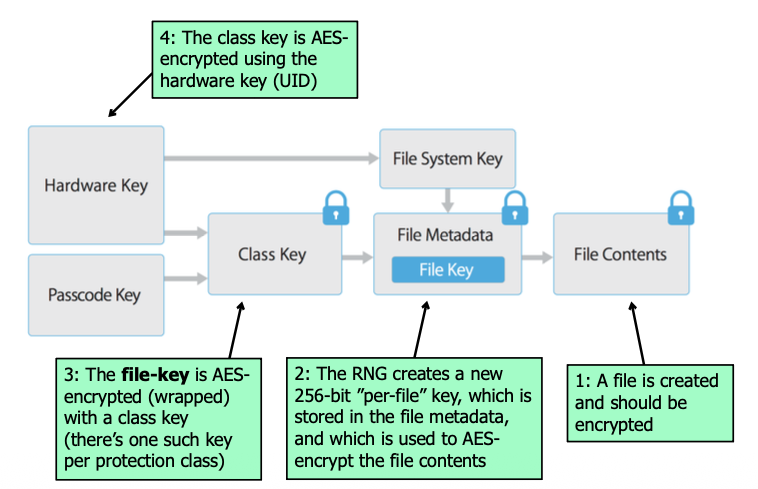
\includegraphics[width=0.9\linewidth]{Figures/file_encryption_ios.png}
\end{center}

% ==================== SECURE ENCLAVE ====================
\section{Secure Enclave \hl{(!)}}
\kw{Hardware key manager}, a \kw{coprocessor isolated} from the main CPU:
\begin{itemize}
\item Own \kw{secure boot chain}, own \kw{AES engine + UID}, separate OS (Apple \kw{L4} microkernel).
\item Stores \kw{fingerprint/face data} \& performs the \kw{match} -- biometric data \kw{never leaves} it.
\item Holds/encrypts \kw{class keys} (e.g. Complete Protection).
\end{itemize}

% ==================== PASSCODES ====================
\section{Passcodes \& Brute Force \hl{(!)}}
4/6-digit or arbitrary \kw{alphanumeric}.
\begin{itemize}
\item Passcode check \kw{entangles passcode with the UID} via AES $\Rightarrow$ must run \kw{on-device} ($\approx$\kw{80\,ms}/try). \hl{No offline brute force} (UID can't be extracted).
\item Ideal brute force: \kw{$\sim$13.5 min} (4-digit) / \kw{$\sim$22 h} (6-digit).
\item Lock-screen \kw{delays}: 5 wrong $\to$1\,min, 9$\to$1\,hr; optional \kw{wipe after 10}.
\item Real attacks: \kw{GrayKey} 2018 ($\sim$72\,h, 2\,h for 4-digit); 2015 iOS 8.1.1 bug (1 try/40\,s).
\end{itemize}

% ==================== DATA PROTECTION CLASSES ====================
\section{Data Protection Classes \hl{(!)}}
Differ in \kw{when the class key is available} (controls \kw{when files can be decryptd}):


{\footnotesize
\setlength{\tabcolsep}{3pt}
\renewcommand{\arraystretch}{1.1}
\arrayrulecolor{zhawblue}
\noindent\begin{tabular}{@{}>{\raggedright\arraybackslash}p{0.30\linewidth}>{\raggedright\arraybackslash}p{0.62\linewidth}@{}}
\rowcolor{zhawblue}
{\color{white}\bfseries Class} & {\color{white}\bfseries Key protection / behaviour}\\
\rowcolor{tableblue}
\kw{Complete Protection} & key = \kw{UID + passcode}; \kw{removed from memory when locked} (e.g. Mail, Health).\\
\rowcolor{white}
\kw{Until First User Auth} & \kw{default} for apps; key stays in memory \kw{after first unlock} (until reboot).\\
\rowcolor{tableblue}
\kw{No Protection} & key = \kw{UID only}; accessible \kw{without passcode} (e.g. Medical ID).\\
\end{tabular}}

\begin{defbox}
\textbf{Exercise (attacker scenarios).} \kw{Alice} = steals + just \kw{possesses} device (locked) $\to$ Complete-Protection files stay safe. \kw{Bob} = steals + makes the user \kw{unlock} it $\to$ everything decryptable. \kw{Carol} = \kw{root exploit} $\to$ reads all class keys currently in memory $\Rightarrow$ all files except locked Complete-Protection. \textit{(Assumes iCloud activation lock bypassed.)}
\end{defbox}

% ==================== TOUCH ID ====================
\section{Touch ID / Face ID}
\begin{itemize}
\item \kw{Fingerprint} unlock; false-accept $\approx$ \kw{1:50{,}000}. A \kw{good fingerprint copy} can break it (non-trivial). Still \kw{better than a 4-digit passcode}.
\item \hl{Passcode required instead of biometrics} (limits attack window): after \kw{restart} or \kw{48\,h} not unlocked, or \kw{5 failed} fingerprint tries.
\item Uses the \kw{Secure Enclave}; \hl{does NOT replace the passcode} -- file encryption still uses the passcode; it's just \kw{more convenient}.
\item Lock/unlock: first unlock (after restart) needs passcode $\to$ \kw{unlocks class key}. When \kw{locking}, Complete-Protection class key is \kw{encrypted by the Secure Enclave} (not deleted) $\Rightarrow$ files temporarily undecryptable; unlock decrypts it again.
\end{itemize}

% ==================== KEYCHAIN ====================
\section{iOS Keychain \hl{(!)}}
Secure store for \kw{passwords \& keys}.
\begin{itemize}
\item Single \kw{SQLite DB} in the FS; \kw{access control} by the kernel \kw{security daemon}.
\item Apps see \kw{only their own entries} -- bound via \kw{App ID} (e.g. \term{A1B2C3D4E5.ch.zhaw.supercoolapp}).
\item Entries use a \kw{data-protection scheme like files}: \kw{Always}(=No Protection, e.g. Find-My token), \kw{AfterFirstUnlock}(=Until First Auth, e.g. Wi-Fi/mail pw), \kw{WhenUnlocked}(=Complete, e.g. most 3rd-party logins).
\item Special classes: \kw{WhenUnlockedThisDeviceOnly} (backed up encrypted via \kw{UID} $\Rightarrow$ \kw{can't restore on another device}); \kw{WhenPasscodeSetThisDeviceOnly} (needs Touch ID/passcode per access, \kw{not backed up at all}).
\end{itemize}
\hl{Limit, not a wall:} \kw{root malware / jailbroken root} can still reach Keychain items.

% ==================== APP CODE SIGNING ====================
\section{App Code Signing \& App Store \hl{(!)}}
Once running, the kernel \kw{controls which apps may run}: only apps \kw{signed by Apple} or \kw{signed via an Apple-issued certificate}.
\begin{itemize}
\item Built-in apps signed \kw{by Apple}; 3rd-party apps signed by the \kw{developer} (must join the \kw{Developer Program} to get a cert).
\item \hl{Extends the chain of trust from OS $\to$ apps}: secure boot guarantees a genuine kernel; kernel knows Apple's root certs \& enforces \kw{signed-only}.
\item 3rd-party install \kw{only via App Store} (exception: \kw{Ad Hoc Provisioning Profile} = limited test devices by UUID).
\item Apple \kw{checks signature} + \kw{reviews} (works "as described", no obvious bugs). Process unclear; \kw{rejects} apps using \kw{private APIs} or that \kw{interpret code} (emulators). Apps \kw{slip through} occasionally $\to$ pulled later.
\end{itemize}

% ==================== SANDBOXING ====================
\section{iOS Runtime Security \& Sandboxing \hl{(!)}}
iOS = based on \kw{OSX} $\to$ \kw{BSD Unix}. Apps in \kw{Objective-C/Swift} compiled to \kw{native code}. Two users: \kw{root} and \kw{mobile}; \hl{all 3rd-party apps run as \kw{mobile}}.
\subsection{App directories (sandbox)}
\begin{itemize}
\item \kw{Bundle Container} (\term{.../Bundle/Application/<AppID>/MyApp.app}): binary + static content, \kw{read-only}, \kw{protected by app signature}.
\item \kw{Data Container}: \kw{Documents} (persistent, e.g. DB; backed up), \kw{Library} (config/prefs/caches/cookies; backed up except Caches), \kw{tmp} (temporary, may be deleted, not backed up).
\item \kw{iCloud} \& other extra containers possible. \term{<AppID>} created \kw{randomly} at install.
\end{itemize}
\subsection{Enforcement -- why MAC, not DAC}
All apps run as \kw{mobile} $\Rightarrow$ \kw{DAC (per-user perms) can't separate them}. iOS uses the \kw{TrustedBSD Mandatory Access Control (MAC)} framework:
\begin{itemize}
\item Per-app \kw{policy file} defines accessible FS parts \& syscalls. Standard policy: \kw{read} Bundle, \kw{read/write} Data container.
\item \hl{Kernel enforces the policy $\Rightarrow$ malicious apps cannot escalate privileges.}
\end{itemize}

\begin{center}
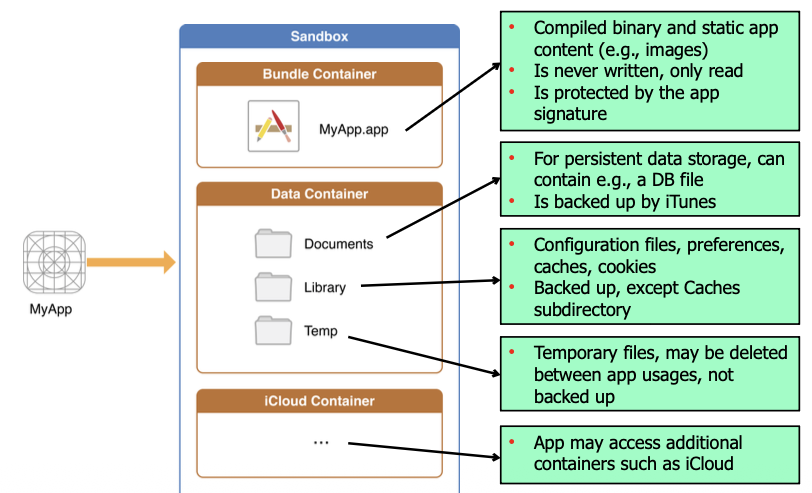
\includegraphics[width=0.9\linewidth]{Figures/sandbox_app_container_ios.png}
\end{center}

% ==================== ADDITIONAL RUNTIME ====================
\section{iOS -- Extra Runtime Defences}
\begin{itemize}
\item \kw{Code Signing Enforcement (CSE)}: code loaded into a page must be \kw{signed}; \hl{no page is both writeable \& executable} (W$\oplus$X) $\Rightarrow$ code can't be modified at runtime.
\item Exception: \kw{Safari / WebViews} get \kw{JIT} (CSE would block code generation).
\item Buffer-overflow defences: \kw{ASLR} (randomise memory layout each launch) + \kw{Execute Never (XN)} ARM feature (stack non-executable).
\end{itemize}

% ==================== PERMISSIONS / INTER-APP ====================
\section{iOS Permissions \& Inter-App}
\begin{itemize}
\item App must \kw{ask the user} to access data/functions (location, camera, contacts, photos\dots) at launch/when needed; \kw{revocable} anytime in settings.
\item \kw{Inter-app} via \kw{URL scheme}: receiver registers a scheme (e.g. \term{zhaw}); sender opens \term{zhaw://...data...} $\to$ receiver brought to foreground, processes it. Receiver may \kw{restrict senders by App ID}. Predefined schemes: \kw{http} (Safari), \kw{tel}, \kw{mailto}.
\end{itemize}

% ==================== JAILBREAKING ====================
\section{Jailbreaking \hl{(!)}}
\kw{Removes iOS protections}, grants \kw{root}. Shouldn't be possible (strong model) -- but \kw{vulnerabilities} give root $\to$ manipulate kernel to disable security. Exploit levels by power:
{\footnotesize
\setlength{\tabcolsep}{3pt}
\renewcommand{\arraystretch}{1.1}
\arrayrulecolor{zhawblue}
\noindent\begin{tabular}{@{}>{\raggedright\arraybackslash}p{0.26\linewidth}>{\raggedright\arraybackslash}p{0.66\linewidth}@{}}
\rowcolor{zhawblue}
{\color{white}\bfseries Level} & {\color{white}\bfseries Power}\\
\rowcolor{tableblue}
\kw{BootROM} & \kw{most powerful}, \kw{cannot be patched} $\to$ modify whole boot chain.\\
\rowcolor{white}
\kw{iBoot} & very powerful, early boot; \kw{fixable by SW upgrade}.\\
\rowcolor{tableblue}
\kw{User space} & weakest, easiest to fix; needs \kw{2 exploits} (code-exec + privilege-escalation).\\
\end{tabular}}
\begin{itemize}
\item \kw{Why}: understand internals, \kw{pentest} apps, install non-App-Store apps, customize, \kw{piracy}. \kw{Cydia}/\kw{Sileo} = the jailbreak "app stores"; install \kw{OpenSSH} for terminal access.
\item \hl{Reduces security a lot}: unsigned apps not sandboxed, root code installable. \kw{Malware risk} much higher -- e.g. \term{IKEE worm} (set wallpaper to Rick Astley) abused the \kw{unchanged default root password "alpine"}.
\item Tethering of jailbreaks: \kw{Untethered} (boots jailbroken alone) / \kw{semi-untethered} (re-JB without PC) / \kw{semi-tethered} (re-JB with PC) / \kw{tethered} (can't even boot without PC). Apple keeps patching; almost all versions \kw{eventually jailbroken}.
\end{itemize}

% ============================================================
%  ANDROID
% ============================================================
\section{Android Security \hl{(!)}}
\kw{Similar features to iOS, but often \kw{less strict} \& \kw{not enforced}}.
\begin{itemize}
\item Reason: runs on a \kw{huge variety of hardware} $\Rightarrow$ e.g. \kw{boot security depends on the device}, not just Android.
\item Features: \kw{sandboxing}, \kw{permission} model, \kw{code signing}, \kw{limited inter-app comm}, \kw{full-disk/file encryption}.
\end{itemize}

% ==================== ANDROID SANDBOXING ====================
\section{Android Runtime \& Sandboxing \hl{(!)}}
Based on a \kw{modified Linux kernel}. Apps in \kw{Java/Kotlin} (native: C/C++). VM: \kw{Dalvik} ($\le$4.4) $\to$ \kw{ART} (5.0+).\\
Build chain: \kw{javac} $\to$ bytecode ($\to$ optional \kw{ProGuard} minify/obfuscate) $\to$ \kw{dx} $\to$ Dalvik bytecode $\to$ at install \kw{dex2oat} $\to$ ART bytecode (\kw{backward compat}).
\subsection{The key idea: \hl{one Linux user per app}}
Apps shipped as \kw{APK/AAB} (zipped bytecode+resources). At install $\to$ \kw{two directories}:
\begin{itemize}
\item \kw{/data/app/ch.zhaw.myapp.apk} -- the APK; owner \kw{system}, \kw{read for everyone} (not sensitive), write = system only.
\item \kw{/data/data/ch.zhaw.myapp/} -- runtime data; a \kw{new dedicated user} (e.g. \term{u0\_a56}) is created \& \kw{owns} it.
\end{itemize}
\subsection{How sandboxing works}
\begin{itemize}
\item App \kw{runs as its own user} (e.g. \term{u0\_a56}); \hl{only that process can read/write its data}. It \kw{can't touch other apps' data} \& vice-versa.
\item \hl{Android uses plain \kw{DAC} (Linux file permissions), \kw{NOT} a MAC model like iOS} -- separation comes from \kw{one UID per app}.
\item Dir perms \term{drwxr-x--x}: others can \kw{enter (x)} but usually \kw{not read} files (used for special inter-app sharing).
\end{itemize}

\section{Android -- Extra Runtime Defences}
Memory-safe Java, \kw{but native C/C++ libs} can still have buffer overflows $\Rightarrow$ \kw{ASLR} (4.0+) + \kw{NX (No eXecute)} on stack/heap.

% ==================== ANDROID PERMISSIONS ====================
\section{Android Permissions \hl{(!)}}
\kw{Fine-grained} model.
\begin{itemize}
\item \kw{Android <6.0}: shown all permissions \kw{at install}, must \kw{accept all} (all-or-nothing).
\item \kw{Android $\ge$6.0}: \kw{normal} (granted implicitly) vs \kw{dangerous} (ask when needed); grouped -- \hl{granting one dangerous perm grants the whole group}.
\item \hl{Users rarely inspect} the list, just hit install $\Rightarrow$ abused by malware (e.g. \kw{overlay attacks}).
\end{itemize}

% ==================== ANDROID CODE SIGNING ====================
\section{Android Code Signing \& Distribution \hl{(!)}}
\hl{Apps can be installed \kw{from anywhere}} (Play Store, e-mail, download) -- untrusted sources are \kw{very risky}.
\begin{itemize}
\item Apps \kw{must be signed}, but \hl{NOT by a Google cert} -- developer uses a \kw{self-signed certificate}. \textit{(Cert: \kw{Issuer == Subject} $\Rightarrow$ self-signed.)}
\item \kw{Purpose} despite self-signed: (1) \kw{update} must be signed with the \kw{same cert} as the previous version (stops a stranger replacing your app); (2) build \kw{trust relationships between apps} signed with the same key.
\item \kw{Play Store doesn't catch all malware}: genuine apps \kw{updated to malicious} later, malware \kw{hides} (e.g. detect emulator), \kw{social engineering}, \kw{APK repackaging} (genuine app repacked with malware).
\end{itemize}

% ==================== ANDROID INTER-APP ====================
\section{Android Inter-App (Intents) \hl{(!)}}
Apps communicate via \kw{intents} sent to a target \kw{activity}.
\begin{itemize}
\item To receive, an activity declares an \kw{intent-filter} in \kw{AndroidManifest.xml} listing accepted \kw{URL schemes} (e.g. \term{zhaw}).
\item Sender uses the scheme (e.g. \term{zhaw://...}); if \kw{multiple apps register the same scheme}, the \kw{user chooses}.
\item vs iOS: \kw{bi-directional} (receiver can reply with an intent); plus \hl{explicit intents} -- name the \kw{fully-qualified activity} (e.g. \term{ch.zhaw.myapp.ReceiverActivity}) $\Rightarrow$ \kw{prevents a malware app hijacking data} by registering many schemes.
\end{itemize}

% ==================== ANDROID ENCRYPTION ====================
\section{Android File Encryption \hl{(!)}}
Supports \kw{Full-Disk (FDE)} \& \kw{File-Based (FBE)}.
{\footnotesize
\setlength{\tabcolsep}{3pt}
\renewcommand{\arraystretch}{1.1}
\arrayrulecolor{zhawblue}
\noindent\begin{tabular}{@{}>{\raggedright\arraybackslash}p{0.16\linewidth}>{\raggedright\arraybackslash}p{0.76\linewidth}@{}}
\rowcolor{zhawblue}
{\color{white}\bfseries Type} & {\color{white}\bfseries Details}\\
\rowcolor{tableblue}
\kw{FDE} & default \kw{Android 5.0--9.0}; \kw{dm-crypt}, \kw{AES-CBC 128-bit} over \term{/data}.\\
\rowcolor{white}
\kw{FBE} & required \kw{Android 10+}; \kw{fscrypt}, \kw{AES-256 XTS}; master key in the \kw{TEE}, unlocked at login.\\
\end{tabular}}
\subsection{Key management}
\begin{itemize}
\item Key \kw{randomly generated} at enable/first boot. \hl{No PIN $\Rightarrow$ key "protected" with literal "default\_password" = no protection.}
\item With PIN/pw: key is \kw{stretched with \kw{scrypt}} then encrypts the FDE key.
\item \hl{"It's complicated"}: vendors modify defaults, TEE may be absent, system apps may not encrypt.
\end{itemize}
\subsection{How it helps vs iOS}
If \kw{device stolen}, most data not easily read. \hl{But unlike iOS the key is \kw{not bound to the hardware}} $\Rightarrow$ attacker can \kw{copy data off the flash} \& brute-force the PIN \kw{with lots of compute} -- \kw{no on-device delays}. \kw{scrypt} makes HW brute force hard, but \kw{short 4/6-digit PINs still crack easily}.

% ==================== ROOTING ====================
\section{Rooting (= Android "Jailbreak") \hl{(!)}}
Goal like jailbreaking: \kw{get root}. Many vendors offer \kw{official ways} (else $\Rightarrow$ vulnerability).
\begin{itemize}
\item Means getting a \kw{su binary} onto the device. \hl{Android root has \kw{no password}} $\Rightarrow$ calling \term{su} (no username) = become root. An app like \kw{SuperSU} pops the \kw{grant/deny} dialog.
\item Two methods: \kw{unlock the bootloader} (flash a pre-rooted kernel with \term{su}) \kw{OR} use a \kw{privilege-escalation vulnerability} (e.g. in the Linux kernel) to install \term{su}.
\item \kw{Why}: see internals, pentest, run \kw{root apps} (backup, debloat). Like JB, \kw{most devices can eventually be rooted}.
\end{itemize}

% ==================== SUMMARY ====================
\section{Summary \hl{(!)}}
\begin{defbox}
\kw{Mobile = different risk profile} (loss, theft, untrusted nets, wallet, 2FA) $\Rightarrow$ OS protections \kw{beyond a PC}. \kw{iOS} = \kw{strong \& restrictive} (secure boot, HW-bound encryption, passcode/Face ID, Keychain, App-Store-only, MAC sandbox, permissions). \kw{Android} = \kw{less restrictive, less secure} (DAC one-user-per-app sandbox, permissions, \kw{apps from anywhere}, intents, FDE/FBE \kw{not HW-bound}). \kw{Jailbreaking (iOS) / rooting (Android)} = grants root, \kw{disables security}, raises malware risk.
\end{defbox}

